\section{BlueShare}\label{blueShare}

BlueShare

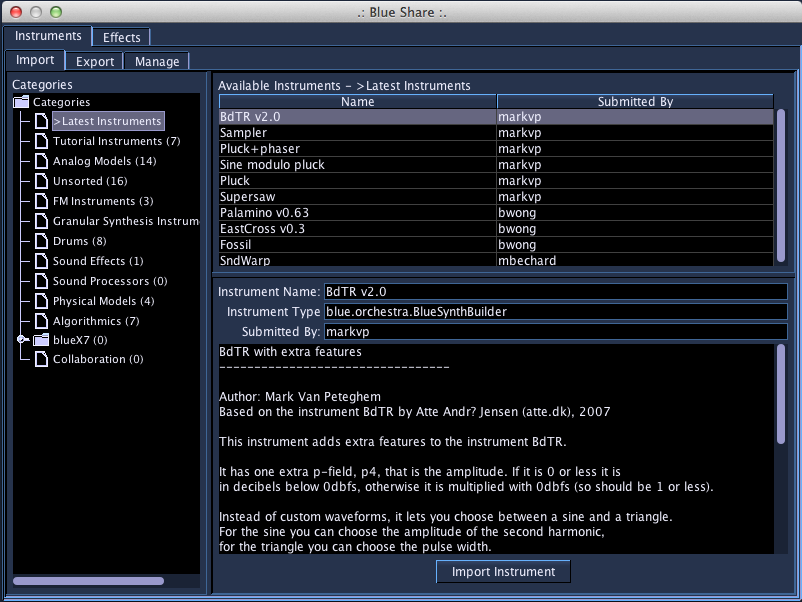
\includegraphics[width=1.00000\textwidth]{images/blueShare.png}

BlueShare is an online, in-program way to share instruments and effects
with other blue users. BlueShare does not require a user account to
download items, but does require one for uploading. If you would like to
share an instrument or effect, please sign up for an account at
\url{http://blue.kunstmusik.com}

To use BlueShare, go to the Tools menu to open it up. Blue will contact
the server to get a list of Instrument and Effects available. From
there, you can browse categories, then select an item in the upper-right
table to get more information. Once you find something you are
interested to try, select "Import Instrument" or "Import Effect". The
instrument or effect will download to your User Instrument Library or
Effects Library in a folder called "Imported Instruments" or "Imported
Effects".

To use BlueShare, go to the Tools menu to open it up. Blue will contact
the server to get a list of Instrument and Effects available. From
there, you can browse categories, then select an item in the upper-right
table to get more information. Once you find something you are
interested to try, select "Import Instrument" or "Import Effect". The
instrument or effect will download to your User Instrument Library or
Effects Library in a folder called "Imported Instruments" or "Imported
Effects".

To upload and instrument or effect, switch to the Export tab. From there
you will see a place to enter your username and password, a listing of
instruments or effects from your libraries, a tree of categories to use
for uploading, and a description box (pre-populated with the Comments
field of your Instrument or Effect). You can then press the "Submit"
button to send it to the server.

The manage tab allows you to pull down a list of your contributed
instruments and effects. You can then remove the item from blueShare
using "Remove" button.
